% Template for ICASSP-2018 paper; to be used with:
%          spconf.sty  - ICASSP/ICIP LaTeX style file, and
%          IEEEbib.bst - IEEE bibliography style file.
% --------------------------------------------------------------------------
\documentclass{article}
\usepackage{spconf,amsmath,amssymb,graphicx,bm,algorithm,algpseudocode,mathtools,xcolor,siunitx}
\graphicspath{{figures/}}

% \newcommand{\R}{\mathbb{R}}
% \renewcommand{\vec}[1]{\ensuremath{\mathbf{#1}}}
% \providecommand{\mat}[1]{\ensuremath{\mathbf{#1}}}
% \providecommand{\vx}{\vec{x}}
% \providecommand{\vy}{\vec{y}}
% \providecommand{\ve}{\vec{e}}
% \providecommand{\vn}{\vec{n}}
% \providecommand{\vA}{\vec{A}}
\providecommand{\norm}[1]{\left\lVert#1\right\rVert}
\DeclareMathOperator*{\argmin}{arg\,min}
\DeclareMathOperator*{\argmax}{arg\,max}

\title{Optimal Measurement Configuration in Computational \\ Diffractive Imaging}

\name{Evan Widloski \qquad Ulas Kamaci \qquad Farzad Kamalabadi}
\address{
Department of Electrical and Computer Engineering and Coordinated Science Laboratory, \\
University of Illinois at Urbana-Champaign, Urbana, IL 61801, USA
}

\begin{document}
\maketitle
% \ninept

\begin{abstract}
% Spectral imaging, forming images of a scene at many wavelengths, is a
% fundamental analysis technique with many scientific applications. Diffractive
% lenses can achieve very high resolution in X-ray and UV regimes as compared to
% reflective and refractive optics. Their wavelength dependent focal length
% enables them to be used in spectral imaging of polychromatic sources, where the
% focused image of each spectral component is formed at different distances from
% the diffractive lens. If measurements are taken at each of these focus
% locations, it is possible to computationally reconstruct the spectral scene by
% solving an inverse problem. In this paper, we propose a greedy algorithm for
% finding a measurement configuration which results in better reconstructions than
% a conventional configuration selection strategy.
% In this paper, we investigate the problem of data acquisition in a multispectral
% diffractive imaging system.  Diffractive systems have the property that the
% spectral components of a polychromatic source are focused at different distances
% from the lens.  This means that in order to image a source at more than one
% wavelength, multiple measurements must be made with a moving detector. However,
% the choice of where to make these measurements is non-obvious and has
% implications on the quality of the reconstructions. Furthermore, an exhaustive
% search of all possible measurement configurations grows exponentially with the
% number of sources and is computationally infeasible. We propose a greedy
% backward elimination algorithm for finding acquisition locations and show that
% reconstruction quality is improved over a naive acquisition strategy.

Diffractive lenses have recently been applied to the domain of multispectral
imaging in the X-ray and UV regimes where they can achieve very high resolution
as compared to reflective and refractive optics. Conventionally, spectral
components are reconstructed by taking measurements at the focal planes.
However, the reconstruction quality can be improved by optimizing the
measurement configuration. In this work, we adapt a sequential backward
selection algorithm to search for a configuration which minimizes expected
reconstruction error. By approximating the forward system as a circular
convolution and making assumptions on the source and noise, we greatly reduce
the complexity of the algorithm. Numerical results show that the configuration
found by the algorithm significantly improves the reconstruction performance
compared to a standard configuration.

\end{abstract}

\begin{keywords}
Spectral imaging, diffractive optics, measurement configuration,
subset selection, computational imaging
\end{keywords}

\section{Introduction}
\label{sec:intro}
Spectral imaging is the formation of images at different wavelengths in the
electromagnetic spectrum. With images usually taken in the visible, X-ray,
ultraviolet (UV), or infrared bands, it has applications in medicine,
geographic surveying, astronomy, and solar physics \cite{shaw2003spectral},
\cite{garini2006spectral}. In spectral imaging, a polychromatic source must be first separated
into its spectral components before being captured. There are a number of ways
to achieve this, but a common method is to use a set of configurable optical
filters. For example, the spectral imager on the Solar Dynamics Observatory uses
a rotating drum of optical filters to selectively pass light of specific
wavelengths of interest \cite{sdo}.

% Spectral imaging is forming images of a scene as a function of wavelength, is a
% fundamental diagnostic technique in various fields such as astronomy,
% surveillance, agriculture and medicine \cite{shaw2003spectral},
% \cite{garini2006spectral}. Forming a three dimensional (3D) data-cube (one
% wavelength and two spatial dimensions) with two dimensional (2D) detector
% measurements can be done by taking multiple exposures. To capture the spectrum
% of a scene, conventional spectral imagers combine regular camera optics with
% either additional wavelength filters or dispersive elements (e.g diffraction
% grating).


A new approach is to use a diffractive lens to perform spectral imaging
\cite{oktem2014icip}.
Diffractive lenses are often preferred in the UV or X-ray regimes because
manufacturing tolerances at these wavelengths can be more relaxed than
reflective optics and still obtain a similar resolution \cite{davila2011high}.
Since diffractive optics can be manufactured using a photolithographic process,
they can be produced at a higher precision compared to the grinding process used
to produce conventional reflective optics. Moreover, refractive optics are
unsuitable for UV or X-ray imaging because glass is opaque at these wavelengths.
Figures \ref{fig:diff_lens}(b) and \ref{fig:diff_lens}(c) are two examples of a
pattern that can be etched into silicon wafer to produce a diffractive lens.


Diffractive lenses have the property that the angle at which light exits the
lens is determined by the light's wavelength, which gives them a wavelength
dependent focal length, as shown in Figure \ref{fig:diff_lens}(a)
\cite{attwood1999}.
% This process forms a focused image of each spectral
% component of source at different distances from the lens \cite{attwood1999}, as
% shown in Figure \ref{fig:diff_lens}(a).


\begin{figure}[htb]

\begin{minipage}[b]{0.48\linewidth}
  \centering
  \centerline{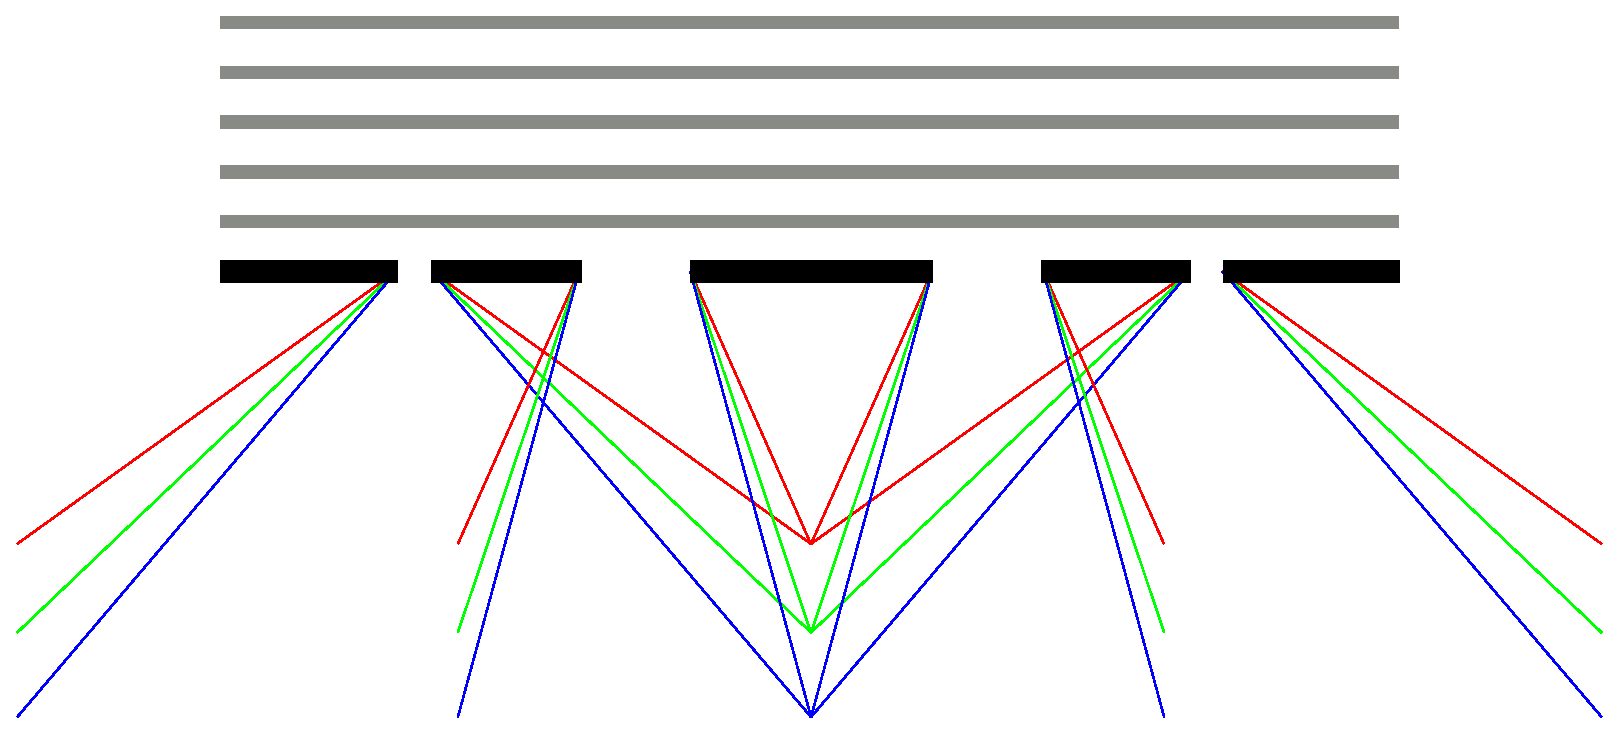
\includegraphics[width=4.0cm]{diffraction_ps_rgb}}
  \centerline{(a)}\medskip
\end{minipage}
\hfill
\begin{minipage}[b]{0.24\linewidth}
  \centering
  \centerline{
\includegraphics[width=2.0cm]{zoneplate.png}}
  \centerline{(b)}\medskip
\end{minipage}
\hfill
\begin{minipage}[b]{0.24\linewidth}
  \centering
  \centerline{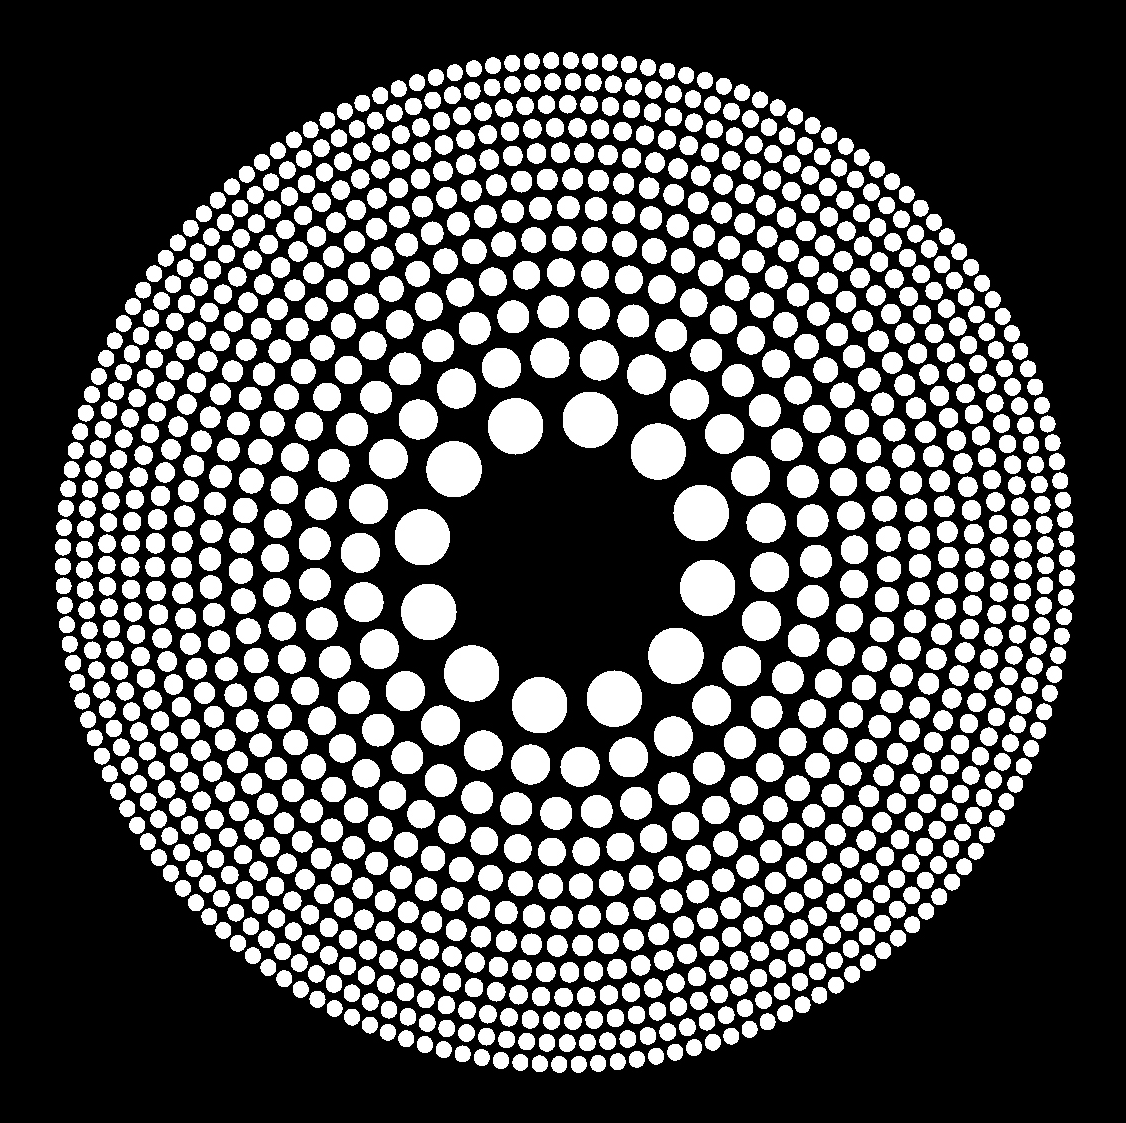
\includegraphics[width=2.0cm]{photonsieve}}
%  \vspace{1.5cm}
  \centerline{(c)}\medskip
\end{minipage}
\caption{(a) diffraction of a polychromatic wave through a diffractive lens (b) Fresnel zone
plate (c) photon sieve \cite{kipp2001sharper}}
\label{fig:diff_lens}
%
\end{figure}

% FIXME
Measurements at the focal plane of each spectral component comprise of a sum of a
focused image of one component and blurred images of all other
components, as shown in Figure \ref{fig:pssi_drawing}.
% Through the process of diffraction, each measurement is actually a sum of all
% spectral components of the source at varying degrees of focus.
An inverse problem consisting of disentangling and deblurring of measurements
must be solved in order to recover the original source components
\cite{oktem2014icip}. However, this focal plane measurement configuration leads
to suboptimal reconstructions, especially when spectral components are close in
wavelength. Therefore, it is desired to determine the optimal measurement
configuration before acquiring the data.

\begin{figure}[htb]
  \begin{minipage}[b]{1\linewidth}
    \centering
    \centerline{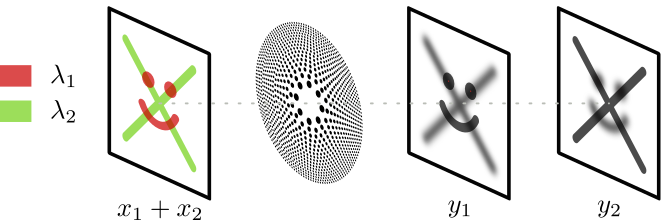
\includegraphics[width=8.5cm]{diffraction_system}}
  \end{minipage}
  \caption{Imaging a scene with emissions at wavelengths $\lambda_1$ and
  $\lambda_2$. Measurements $y_1$ and $y_2$ are taken at two positions where one wavelength
  is in focus and the other is out of focus.}
  \label{fig:pssi_drawing}
\end{figure}


Finding the optimal measurement configuration can be seen as a \emph{sensor
placement problem}, which lies under the broader class of problems known as
\emph{subset selection}. Subset selection applies to many domains, such as array
optimization for atmospheric imaging \cite{sharif}, \cite{wang2017near},
magnetic resonance imaging \cite{gao2000optimal}, and detection problems
\cite{yu1997sampling}. Methods like genetic algorithms, convex optimization
\cite{joshi2008sensor}, and hill climbing \cite{reeves1999sequential} with many
selection criteria have been developed to solve such problems.


However, most of these methods solve the problem of
single-sensor/single-measurement systems where the placement of one sensor
contributes a single row to the observation matrix. In contrast, many imaging
systems are single-sensor/multiple-measurement (like our problem), where each sensor placed (measurement plane) contributes multiple rows to the observation matrix (one row
per detector pixel). Single-sensor/single-measurement algorithms have been
extended to the multiple measurement case, known as \emph{clustering}
algorithms. Examples include \emph{clustered sequential backward selection} (CSBS)
\cite{sharif}, \emph{clustered FrameSense} (CFS) \cite{ranieri2014near}, \emph{clustered maximum projection on minimum eigenspace} (CMPME) \cite{wang2018sampling}.

% Finding the optimal measurement configuration can be seen as a sensor placement
% problem, which lies under the broader class of problems known as subset
% selection. It appears in many signal reconstruction problems in the domains of
% sensor networks [?], magnetic resonance imaging [?], remote sensing [?] ...
% Many selection algorithms that have been developed are based on greedy search
% [?] or convex optimization [?]. Of these methods, we are interested in the ones
% that consider the case where each sensor location contributes to multiple
% measurements. Clustered sequential backward selection (CSBS) \cite{sharif},
%  .
%
% - explain how the problem is sensor placement
% - sensor placement ---> subset selection
% - other problems with subset selection [...]
% - methods to find optimal subset for single row
% - single row is limited, formulation needs to be extended to capture clusters
% - Cite CSBS CMPME CFS and Boyd's paper
% - We studied CSBS, provided speed-up and obtained performance improvement

% In fact, any plane consists of a sum of all spectral
% components of the source at varying degrees of focus, which depends on the
% distance from lens and the wavelenght. Then a strategy to perform spectral
% imaging is to take a measurement at each focal plane and solve an inverse
% problem consisting of disentangling and deblurring of measurements in order to
% recover the original spectral components \cite{oktem2014icip}. Considering the
% fact that each measurement will contain noise, deblurring problem will be ill
% posed. Furthermore, the inverse problem becomes more ill posed if the wavelengths
% of interest are very close to each other, because it gets harder to disentangle.

% In an ill posed problem like this, the choice of measurement planes becomes very
% crucial and has direct impact on the reconstruction quality. Although taking
% many measurements, or choosing longer exposure time will make the problem more
% well posed, practical applications usually impose limits on the total
% measurement time due to the dynamics of the scene. Even if there is no time
% limitation, given the freedom to take $M$ measurements out of $C$ candidate
% plane locations, it is desired to find the best configuration that maximizes the
% reconstruction quality.

In this paper we adapt CSBS to the diffractive imaging problem to automatically
determine a measurement configuration from a set of candidate plane locations,
which minimizes expected reconstruction error. Furthermore, we exploit
structures in the imaging model to make the algorithm computationally feasible
for large images.
% Exploiting the
% structures of the imaging model, we have implemented the algorithm efficiently,
% which otherwise would be infeasible to implement.

% In the next section, we mathematically model the diffractive imaging system and
% formulate the inverse problem of recovering spectral components. In Sections 3
% and 4 we describe the measurement selection algorithm and show a fast
% implementation. Next, the complexity of the fast implementation is analysed and
% compared with the complexity of the general algorithm. The last section is
% dedicated to a numerical analysis demonstrating the improved reconstruction
% quality when the algorithm is used to select a measurement configuration.

% A different approach is to use a diffractive lens to perform spectral imaging.
% Diffractive lenses focus light using the diffraction principle. They have
% wavelength dependent focal length which is the property that enables them to be
% used as spectral imagers (see Figure \ref{fig:diff_lens}). Examples of
% diffractive lenses are Fresnel zone plates and their modifications (e.g. photon
% sieve) (see Figure \ref{fig:diff_lens}). Diffractive lenses are preferred in
% applications in UV and X-ray regimes where they can provide high resolution
% whereas reflective optics are very costly to manufacture to achieve high
% resolution and refractive lenses cannot be used due to light absorption in these
% regimes.


% Photon sieve spectral imaging (PSSI) is a modality that takes the advantage of
% the wavelength dependent focal length of a photon sieve to perform high
% resolution spectral imaging \cite{oktem2014icip}. It takes multiple exposures of
% the scene at different distances from the lens. Figure \ref{fig:pssi_drawing}
% illustrates the PSSI measurements for a scene radiating at two wavelengths
% $\lambda_1$ and $\lambda_2$. Each measurement consists of blurred superposition
% of the spectral images. The spectral images are then reconstructed from these
% measurements by solving a multi-frame deconvolution problem.


% Choice of measurement planes is an important factor affecting the reconstruction
% quality of the spectral images. Where to take measurements to maximize the
% fidelity of the reconstructions?

% One way is to scan the
% wavelength dimension by using color filters with narrow bandpass to filter
% desired wavelengths at each exposure. Another way is to capture the whole
% spectrum of a portion of the scene at an exposure, and scan a spatial dimension.
% In both methods, the 3D data-cube is then simply reconstructed by stacking the
% 2D measurements in the scanning dimension.

% There are also computational methods which rely on signal processing methods and
% computational power to improve upon the conventional methods in terms of spatial
% and spectral resolutions, total exposure time etc. They utilize more
% sophisticated image acquisition techniques than the conventional scanning-based
% methods, and computationally reconstruct the data-cube from multiplexed/encoded
% measurements. Such methods include compressive coded aperture snapshot spectral
% imaging (CASSI) [REF], compressive hyperspectral imaging by separable spectral
% and spatial operators (CHISS) [REF], and photon sieve spectral imaging (PSSI)
% \cite{oktem2014icip}.

% We will use PSSI as an example modality to explain and demonstrate our work
% because it  uses a diffractive lens, and it is a computational spectral imaging
% modality \cite{oktem2014icip}. Photon sieves, just like Fresnel zone plates, are
% diffractive lenses that use diffraction phenomenon to focus light. Diffractive
% lenses are preferred in applications in UV and X-ray regimes since they can
% provide high resolution whereas reflective optics are very costly to manufacture
% to achieve high resolution and refractive lenses cannot be used due to light
% absorption. They have wavelength dependent focal length which is what behind the
% working principle of PSSI. It takes multiple exposures at different distances
% from the lens to sample the measurement space.

\section{Forward Model and Statistical Formulation}
\label{sec:format}
In this section, we mathematically model a diffractive imaging system and
describe the process of recovering the spectral components. Consider a
polychromatic source that has $S$ spectral components $\bm{x}_1, \dots,
\bm{x}_S \in \mathbb R^{N_1\times N_1}$. Using a moving detector, we make $M$ measurements $\bm{y}_1, \dots,
\bm{y}_M \in \mathbb R^{N_2\times N_2}$ at distances $d_1, \dots, d_M$ from the lens. We allow for repeated
measurements at the same plane for a more flexible model that can take into
account non equal exposure times.
% FIXME
Due to linearity, each measurement is a superposition of blurred versions of the
$S$ sources. More formally,

\begin{equation}
\bm{y}_m = \sum_{s=1}^S \bm{a}_{m,s} \ast \bm{x}_s + \bm{n}_m
\label{eq:fwd_model}
\end{equation}

where $\bm{a}_{m,s} \in \mathbb R^{P\times P}$ is a blurring kernel known as a
\emph{point spread function} (PSF), $\ast$ is a 2D convolution, and $\bm{n}_m
\in \mathbb R^{N_2 \times N_2}$ is additive measurement noise. Each PSF depends
on the associated source wavelength and measurement location together with the
diffractive lens parameters and can be computed efficiently
\cite{ayazgok2020efficient}.
% An example set of PSF images for $M=S=2$ case is given in Figure \ref{fig:psfs}.

Since convolution is a linear operation, we can rewrite the above equation as a
linear system

\begin{equation}
  \underbrace{
    \begin{bmatrix}\bm{y}_1 \\ \vdots \\ \bm{y}_M\end{bmatrix}
  }_{\bm{y}}
  =
  \underbrace{
    \begin{bmatrix}
      \bm{A}_{1, 1} & \hdots & \bm{A}_{1, S} \\
      \vdots & & \vdots \\
      \bm{A}_{M, 1} & \hdots & \bm{A}_{M, S}
    \end{bmatrix}
  }_{\bm{A}_{\bm{d}}}
  \underbrace{
    \begin{bmatrix}\bm{x}_1 \\ \vdots \\ \bm{x}_S\end{bmatrix}
  }_{\bm{x}}
  +
  \underbrace{
    \begin{bmatrix}\bm{n}_1 \\ \vdots \\ \bm{n}_M\end{bmatrix}
  }_{\bm{n}}
\label{eq:fourier_mtx}
\end{equation}

% \begin{figure}[htb]
%   \begin{minipage}[b]{1\linewidth}
%     \centering
%     \centerline{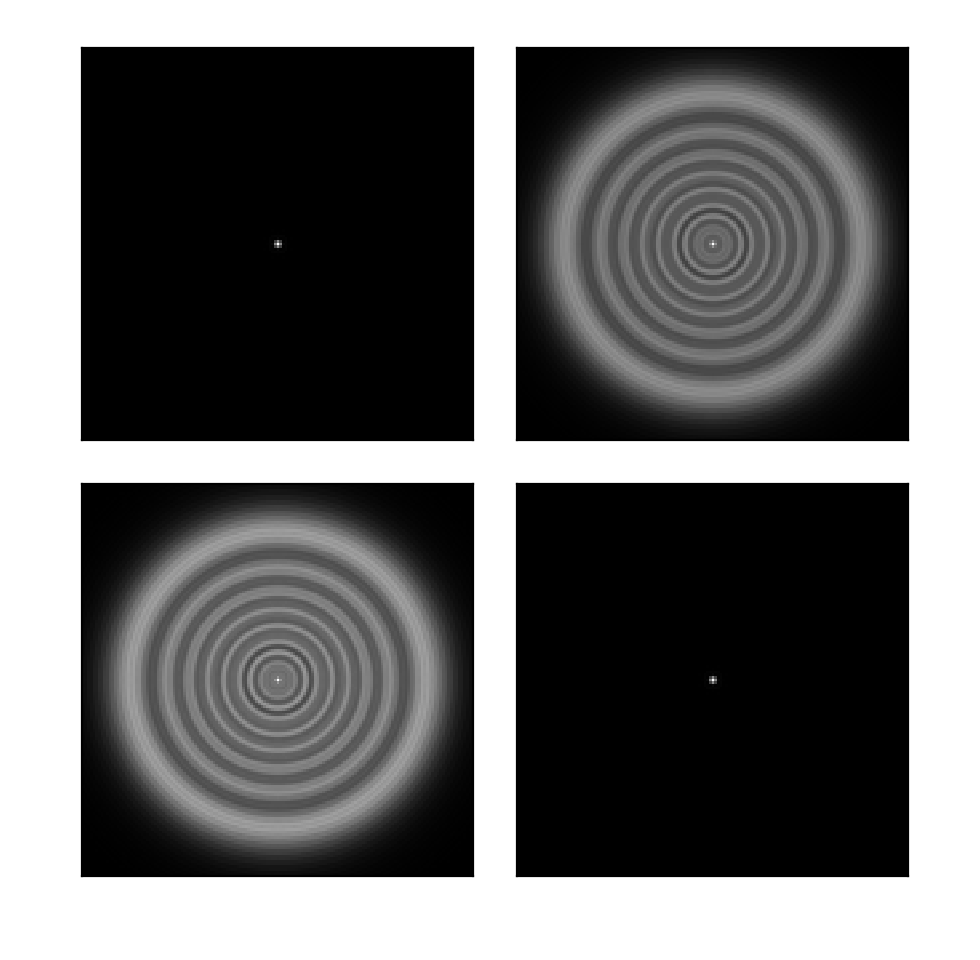
\includegraphics[width=5cm]{psfs}}
%   \end{minipage}
%   \caption{Example point spread functions for measuring a source with 2 spectral
%     components at the focal planes of each component.}
%   \label{fig:psfs}
% \end{figure}

where $\bm{y}_m \in \mathbb R^{N_2^2\times 1}$, $\bm{x}_s \in \mathbb R^{N_1^2\times 1}$ and $\bm{n}_m \in \mathbb R^{N_2^2\times 1}$ have been flattened from their
original 2D shape, and each $\bm{A}_{m,s} \in \mathbb R^{N_2^2\times N_1^2}$ is a block-toeplitz
matrix with toeplitz blocks formed from 2D convolution with PSF $\bm{a}_{m,s}$.
We will refer to the matrix containing all $\bm{A}_{m,s}$
generated by measurements taken at $\bm{d} = \{d_1, \dots, d_M\}$ as
$\bm{A}_{\bm{d}}$.

The problem of where to take measurements $\bm{y}_1, \dots, \bm{y}_M$ has not
been addressed and affects the reconstruction quality.  In order to compare the
impact of different measurement configurations on the reconstruction, it is
necessary to define some cost for the measurement matrix $\bm{A}_{\bm{d}}$.  A
common cost metric is the expected reconstruction error, or expected \emph{sum
of squared errors} (SSE). However, we must have some strategy for the recovery
of $\bm{x}$ to get reconstruction error and we must make statistical assumptions
about $\bm{x}$.\emph{ Maximum a posteriori} (MAP) estimation is one such
strategy.

We assume the original spectral components and noise are distributed according to a
normal distribution such that $\bm{x} \sim \mathcal{N}(\bm{x}_{0}, \bm{\Sigma}_{\bm{x}})$ and
$\bm{n} \sim \mathcal{N}(0, \bm{\Sigma}_{\bm{n}})$.  The MAP estimate is then

% FIXME - dimensionality -> n
% use A instead of H?
$$
\begin{aligned}
  \bm{x}_{MAP} &= \arg \max_{\bm{x} \in \mathbb{C}^n} p(\bm{x} | \bm{y})
  = \arg \max_{\bm{x}} p(\bm{y}|\bm{x}) p(\bm{x})\\
  &= \arg \min_{\bm{x}} \left[  - \log(p(\bm{y}|\bm{x})) - \log
  p(\bm{x})\right] \\
  &= \bm{x}_0 + \left( \bm{A}_{\bm{d}}^H\bm{\Sigma}_{\bm{n}}^{-1} \bm{A}_{\bm{d}} +
    \bm{\Sigma}_{\bm{x}}^{-1}\right)^{-1}
  \cdot  \bm{A}_{\bm{d}}^H \bm{\Sigma}_{\bm{n}}^{-1} (\bm{y} - \bm{A}_{\bm{d}} \bm{x}_0)
\end{aligned}
$$
The reconstruction error is defined as $\bm{e} = \bm{x} - \bm{x_{\text{MAP}}}$,
and the expected sum of squared error cost is $E[\norm{\bm{e}}_2^2]$. This
expression can be rewritten in terms of the error covariance:

\begin{align*}
\mathbb{E}[\norm{\bm{e}}_2^2] =  \mathbb{E}[\bm{e}^H\bm{e}] & = \mathbb{E}[\text{tr}(\bm{e}^H\bm{e})] = \mathbb{E}[\text{tr}(\bm{e}\bm{e}^H)] \\
& = \text{tr}(\mathbb{E}[\bm{e}\bm{e}^H]) = \text{tr}(\bm{\Sigma}_{\bm{e}})
\end{align*}

where the error covariance matrix is defined as $\bm{\Sigma}_{\bm{e}} =
E[\bm{e}\bm{e}^H]$ and has the closed form expression:
\begin{equation}
\bm{\Sigma}_{\bm{e}} = \left( \bm{A}_{\bm{d}}^H\bm{\Sigma}_{\bm{n}}^{-1} \bm{A}_{\bm{d}} +
    \bm{\Sigma}_{\bm{x}}^{-1}\right)^{-1}
\end{equation}

Combining the above equations, we can now write a cost metric which lets us evalute
the expected reconstruction error for a particular measurement configuration $\bm{d}$:
\begin{equation}
\text{Cost}(\bm{d}) = \mathbb{E}[\norm{\bm{e}}_2^2] = \text{tr}\left(\left( \bm{A}_{\bm{d}}^H\bm{\Sigma}_{\bm{n}}^{-1} \bm{A}_{\bm{d}} +
    \bm{\Sigma}_{\bm{x}}^{-1}\right)^{-1}\right)
\end{equation}

% In this section, we mathematically model a multispectral diffractive imaging system.
% Consider a polychromatic source that has spectral emissions at $S$ distinct
% wavelengths $\lambda_1, \dots, \lambda_S$. Using a moving detector,
% we take measurements at $M$ different measurement planes, with distances from the
% sieve $d_1, \dots, d_M$ (see Figure \ref{fig:meas}).  Each of these $M$
% measurements is a sum over the $S$ sources, with each source blurred to varying
% degrees.

% With this,
% the discrete model that relates the noiseless measurements to the sources is
% given by the following model:
% \begin{equation}
% y_k[m,n] = \sum_{p=1}^P h_{d_k,\lambda_p}[m,n] \ast x_p[m,n] \ , \ k = 1,2,\dots, K
% \label{eq:fwd}
% \end{equation}
% where $m,n=-N/2, \dots, N/2-1$ assuming that the detector has $N\times N$
% pixels. Here, $x_p$ denotes the discretized intensity of the source with
% wavelength $\lambda_p$, and $h_{d_k,\lambda_p}$ denotes the discretized point
% spread function (PSF) of the photon sieve for the wavelength $\lambda_p$ and
% plane distance $d_k$, which has a closed form expression given in
% \cite{oktem2013icip}. So, each measurement $y_k$ is a superposition of all the
% sources $x_p$ convolved with their corresponding PSFs $h_{d_k,\lambda_p}$.

% \begin{figure}[h]
% 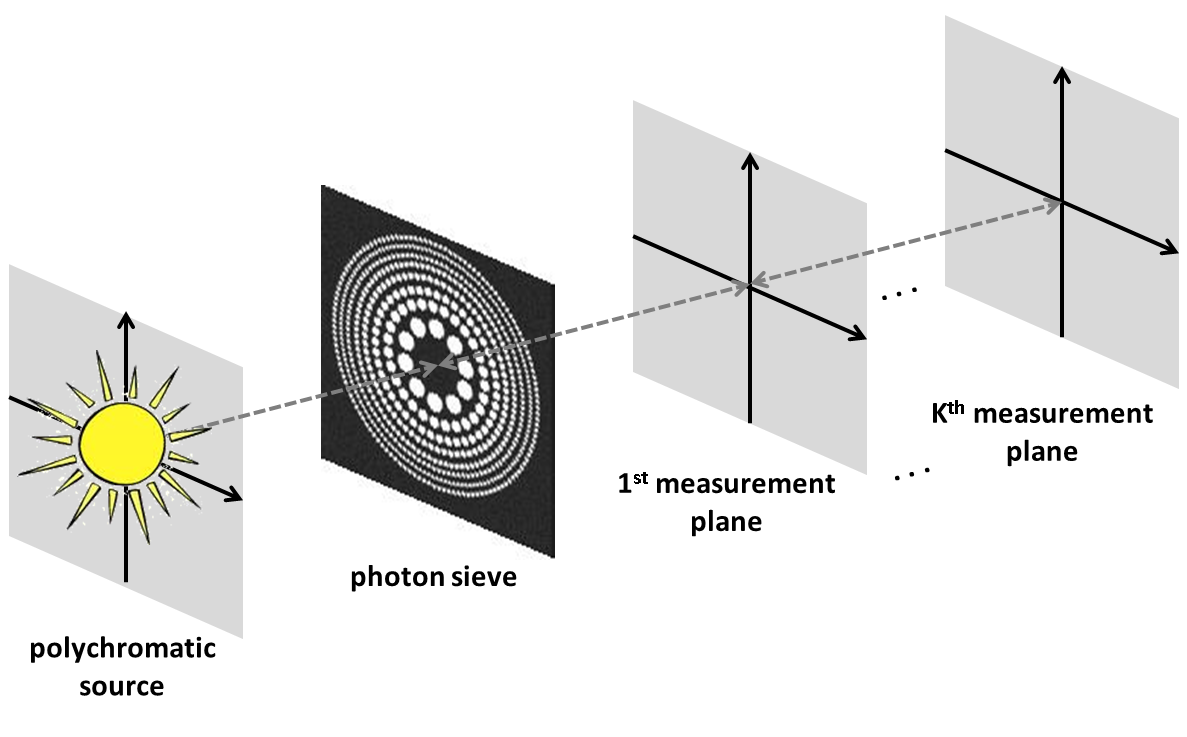
\includegraphics[width=0.45\textwidth]{poster1}
% \caption{PSSI measurement configuration.}
% \label{fig:meas}
% \end{figure}


% Since \eqref{eq:fwd} is a linear relation between the sources and the
% measurements, we can represent it using matrix-vector form which will be useful
% in formulating the inverse problem. Denote by $\vx_p$ and $\vy_k$ the vectorized
% versions of $x_p[m,n]$ and $y_k[m,n]$. Then, we have
% \begin{equation}
% \vy = \vec A \vx + \vec w
% \label{eq:mtx-vec}
% \end{equation}
% with
% \begin{equation}
% \vy = \begin{bmatrix}
% \vy_1 \\ \vdots \\ \vy_K
% \end{bmatrix}, \vA = \begin{bmatrix}
% \vA_{11} \hspace{-.1 in}& \dots \hspace{-.1 in}& \vA_{1P} \\
% \vdots \hspace{-.1 in}& \ddots \hspace{-.1 in}& \vdots \\
% \vA_{K1} \hspace{-.1 in}& \dots \hspace{-.1 in}& \vA_{KP}
% \end{bmatrix}, \vx = \begin{bmatrix}
% \vx_1 \\ \vdots \\ \vx_P
% \end{bmatrix}, \vw = \begin{bmatrix}
% \vw_1 \\ \vdots \\ \vw_K
% \end{bmatrix}
% \end{equation}

% where $\vw_k \in \R^{N^2}$ is additive Gaussian noise vector with $(\vw_k)_i
% \sim \mathcal N (0, \sigma_k^2)$; and $\vA_{k,p} \in \R^{N^2 \times N^2}$ is the
% convolution matrix corresponding to the PSF $h_{d_k,\lambda_p}$. We assume that
% the periodic boundary conditions hold, which makes the matrices $\vA_{k,p}$
% block circulant with circulant blocks (BCCB). This allows computationally
% efficient algorithms in the image reconstruction.


\section{Measurement Selection Algorithm}

With a method of evaluating the effect a particular configuration $\bm{d}$ has
on reconstruction error, we can begin considering which configurations are best
suited for minimizing error.  For example, if we are provided with a set of $C$
candidate measurement locations, we may wish to find a subset of size $M$ which
minimizes reconstruction error. This is known as a \emph{subset selection} problem.
One might think to simply search over all possible measurement configurations
of size $M$, but this exhaustive search requires $\binom{C}{M}$ evalutions of
cost, growing on the order of $O(C^M)$.
% With a method of comparing the *** of two measurement configurations, one might
% think to simply search all possible measurements and choose the best.  However,
% the computational cost of an exhaustive search grows too quickly and is
% infeasible for most realistic scenarios.  For example, consider a scenario in
% which there are $C$ candidate measurement locations of which we would like to
% select a subset of size $M$ to form our measurement matrix $\bm{A}$.
% Exhaustively searching through all possible configurations of $\bm{A}$ would
% require $\binom{C}{M}$ iterations, recomputing $\text{Cost}(\bm{A})$ each time.

CSBS is an alternative method which is more computationally feasible, where one
measurement location is eliminated from $\bm{d}$ in each iteration until only
$M$ locations remain. As reconstruction error generally increases as the number
of measurements decreases, CSBS selects for elimination the measurement that
incurs the smallest increase in cost in each iteration.

\begin{algorithm}
  \begin{algorithmic}
    \caption{CSBS Algorithm}
    \State $\bm{d} = \{d_1, \dots, d_C\}$
    \Repeat
      \State $d' = \arg \min_{d \in \bm{d}} \text{Cost}(\bm{d} \backslash \{d\}))$
      \State $\bm{d} = \bm{d} \backslash \{d'\}$
    \Until{$|\bm{d}| = M$}
  \end{algorithmic}
\end{algorithm}

Unlike an exhaustive search, the complexity of CSBS is not combinatorial.  As the
size of $\bm{d}$ shrinks with each iteration, the number of cost evaluations for each
minimization step decreases.  The total number of cost evaluations is
\vspace{-0.1 in}
$$
\begin{aligned}
  \sum_{|\bm{d}| = M}^C |\bm{d}|
  % &= \frac{C
  %   (C + 1)}{2} - \frac{M(M + 1)}{2} \\
  &= O(C^2 - M^2)
\end{aligned}
$$

% Having defined the cost metric, we are now looking for the best measurement
% configuration to minimize the cost. Suppose we take $M$ measurements, each at
% a distance $d_m$ from the lens for $m = 1, \dots, M$.

% \begin{equation}
% \hat {\bm A} = \argmin_{\vA \in Q} \ \text{Cost}(\bm{A})
% \label{eq:inverse}
% \end{equation}
% The goal in the inverse problem is to reconstruct the spectral components
% $\bm{x}_1, \dots, \bm{x}_S$ from the noisy, blurry and superimposed measurements
% $\bm{y}_1, \dots, \bm{y}_M$. This is known as a \emph{multi-frame deconvolution
% problem} with multiple sources.  However, deconvolution is known to be highly
% ill-posed, which means that direct inversion of the matrix containing the PSFs
% (or its least square approximation) amplifies the noise in the measurements and
% leads to poor reconstructions. To avoid noise amplification, the problem needs
% to be regularized. The inverse problem can then be formulated as a regularized
% optimization problem as follows:
% \begin{equation}
% \hat \vx = \argmin_{\vx} \norm{\vA\vx-\vy}_2^2 + \lambda \mathcal R(\vx)
% \label{eq:inverse}
% \end{equation}
% where the first term ensures that the reconstructions comply with the
% measurements and the second term is the regularization term with parameter
% $\lambda>0$. In this paper, we are interested in

\vspace{-0.1 in}
\section{Fast Implementation}
While the SSE cost applies to any general linear system, we can augment the
complexity reduction achieved by CSBS by making assumptions about the structure
of $\bm{A}_{\bm{d}}$, $\bm{\Sigma}_{\bm{n}}$ and $\bm{\Sigma}_{\bm{x}}$.
Specifically, if we assume the blocks of these matrices are block-circulant with
circulant blocks (BCCB), then they can be diagonalized by the 2D DFT matrix
where operations involving multiplications and inversions are much faster.

For $\bm{A}_{\bm{d}}$ this means that each block $\bm A_{m,s}$ is BCCB and
corresponds to circular convolution with the kernel $\bm a_{m,s}$. For $\bm
\Sigma_n$, we assume independent noise among image pixels and measurement planes
with variance $(1/\lambda)$, so $\bm \Sigma_n=(1/\lambda) \bm I$ where $\bm I$
represents the identity matrix. For $\bm \Sigma_x$, each of its blocks being
BCCB means that the covariance among image pixels are represented by 2D
convolution kernels.

Assuming $N \times N$ images, each $N^2 \times N^2$ block $\bm A_{m,s}$ of $\bm
{A_d}$ can be decomposed as $\bm A_{m,s} = \bm F^{-1} \widetilde{\bm A}_{m,s}
\bm F$ where $\widetilde{\bm A}_{m,s}$ is the diagonal matrix consisting of the
2D DFT of $\bm a_{m,s}$, and $\bm F$ is the 2D DFT matrix. This yields
\vspace{-0.1 in}
\begin{equation}
  \bm {A_d}=
  \underbrace{
    \begin{bmatrix}
      \bm F^{-1} \hspace{-0.2 in}& \hspace{-0.2 in} & \hspace{-0.20 in} \vspace{-0.1 in}\text{\Large 0} \\
        \vspace{-0.05 in}&\hspace{-0.20 in} \ddots &  \\
      \text{\Large 0} \hspace{-0.17 in}& \hspace{-0.2 in} & \hspace{-0.15 in} \bm F^{-1}
    \end{bmatrix}
  }_{\widetilde{\bm F}^{-1}}
  \underbrace{
    \begin{bmatrix}
      \widetilde{\bm A}_{1,1} \hspace{-0.1 in}&\hspace{-0.1 in} \hdots & \hspace{-0.1 in} \widetilde{\bm A}_{1,S} \vspace{-0.02 in}\\
      \vspace{-0.02 in}\vdots &\hspace{-0.1 in} \ddots& \vdots \\
      \widetilde{\bm A}_{M,1} \hspace{-0.1 in}&\hspace{-0.1 in} \hdots & \hspace{-0.1 in} \widetilde{\bm A}_{M,S} \\
    \end{bmatrix}
  }_{\widetilde{\bm A}_{\bm d}}
  \underbrace{
    \begin{bmatrix}
      \bm F \hspace{-0.1 in}& & \hspace{-0.18 in} \vspace{-0.1 in}\text{\Large 0} \\
        \vspace{-0.05 in}& \hspace{-0.12 in}\ddots &  \\
  \hspace{0.05 in} \text{\Large 0} & & \hspace{-0.12 in} \bm F
    \end{bmatrix}
  }_{\widetilde{\bm F}}
\label{eq:fourier_mtx}
\end{equation}
\vspace{-0.1 in}

so, we have $\bm{A_d} = \widetilde{\bm F}^{-1} \widetilde{\bm A}_{\bm d}
\widetilde{\bm F}$, from which we get $\bm{A_d}^H \bm{A_d} = \widetilde{\bm
F}^{-1} \widetilde{\bm A}_{\bm d}^H \widetilde{\bm A}_{\bm d} \widetilde{\bm
F}$. Applying the same procedure, we get $\bm \Sigma_x^{-1} =
\widetilde{\bm F}^{-1} \widetilde{\bm \Sigma}_x^{-1} \widetilde{\bm F}$.
The SSE cost for a measurement configuration $\bm d$ then becomes (scaling both terms
with $\lambda$):
\begin{align}
\text{Cost}(\bm{d}) & = \text{tr}\left(\left( {\bm A}_{\bm d}^H {\bm A}_{\bm d} +
\lambda \bm \Sigma_x^{-1} \right)^{-1} \right)
\label{eq:naive_cost}\\
% & = tr\left(\left(\widetilde{\bm F}^{-1} \widetilde{\bm
% A}_{\bm d}^H \widetilde{\bm A}_{\bm d} \widetilde{\bm F} + \lambda \widetilde{\bm
% F}^{-1} \widetilde{\bm D}^H \widetilde{\bm D} \widetilde{\bm
% F}\right)^{-1}\right) \nonumber \\
& = \text{tr}\left(\left(\widetilde{\bm F}^{-1} \left( \widetilde{\bm A}_{\bm d}^H
\widetilde{\bm A}_{\bm d} + \lambda \widetilde{\bm \Sigma}_x^{-1} \right)
\widetilde{\bm F}\right)^{-1}\right) \nonumber \\
& = \text{tr}\left(\widetilde{\bm F}^{-1} \left( \widetilde{\bm A}_{\bm d}^H
\widetilde{\bm A}_{\bm d} + \lambda \widetilde{\bm \Sigma}_x^{-1} \right)^{-1}
\widetilde{\bm F}\right) \nonumber \\
& = \text{tr}\left(\left( \widetilde{\bm A}_{\bm d}^H \widetilde{\bm A}_{\bm d} +
\lambda \widetilde{\bm \Sigma}_x^{-1} \right)^{-1} \right)
\label{eq:fast_cost}
\end{align}
where the computational complexity of evaluating \eqref{eq:fast_cost} is much
less than \eqref{eq:naive_cost} due to the diagonalized blocks of
$\widetilde{\bm A}_{\bm d}$ and $\widetilde{\bm \Sigma}_x^{-1}$.

There are two contributors to the complexity of evaluating the cost at
$\text{Cost}(\bm{d})$ for a particular configuration: The multiplication
$\widetilde{\bm A}_{\bm d}^H \widetilde{\bm A}_{\bm d}$, and the inversion
$\left( \widetilde{\bm A}_{\bm d}^H \widetilde{\bm A}_{\bm d} + \lambda
\widetilde{\bm \Sigma}_x^{-1} \right)^{-1}$. In fact, the product
$\widetilde{\bm A}_{\bm d}^H \widetilde{\bm A}_{\bm d}$ only needs to be
calculated once during the algorithm initialization, and it can be efficiently
updated at each iteration by adding/subracting the contribution of the candidate plane
that is iterated over, which can be precomputed.

Thus, the complexity of overall CSBS algorithm is dominated by the inversion
of $\left( \widetilde{\bm A}_{\bm d}^H \widetilde{\bm A}_{\bm d} +
\lambda \widetilde{\bm \Sigma}_x^{-1} \right) \in \mathbb C ^{SN^2 \times SN^2}$
that is performed in each iteration.  While the complexity of a standard inversion algorithm
is $O((SN^2)^3)$, the diagonal structure of this matrix allows for a much faster inversion algorithm
with complexity $O(S^3N^2)$, a speed-up of $N^4$ which is significant for large images.

The total CSBS algorithm complexity is
\vspace{-0.1 in}
$$
O_{sbs} = \sum_{|\bm{d}| = M}^C |\bm{d}| O(S^3N^2) = O(S^3N^2C^2)
$$


% Complexity of a standard inversion
% algorithm would give $O_i \triangleq O((SN^2)^3) = O(S^3N^6)$. However, the
% diagonal structure in $\bm \Psi$ allows for a much faster inversion algorithm
% of complexity $O_i = O(S^3N^2)$ \cite{kamaci2017}, providing a speed-up of $N^4$, which is significant for large image sizes. The total complexity of the CSBS algorithm can
% be written as:
% $$
% O_{sbs} = \sum_{|\bm{d}| = M}^C |\bm{d}| O_i = O(S^3N^2C^2)
% $$

% \section{Complexity Analysis}
%
% In this section, we derive the computational complexity of the general
% CSBS implementation and our fast version as a function of the number of pixels
% in an image $N^2$, the number of spectral components $S$ in the source, and the
% number of candidate measurement locations $C$.
%
% \subsection{General Implementation Complexity}
%
% The computational complexity of evaluating cost for a particular measurement
% configuration $\bm{d}$ comes from two places in the cost formulation.
%
% \vspace{-0.2 in}
% $$
%   \text{Cost}(\bm{d}) = \text{tr} \Bigl(
%   \overbrace{\vphantom{\rule[1.5em]{0pt}{0pt}}
% (\underbrace{\vphantom{\rule[-0.5em]{0pt}{0pt}} \bm{A}_{\bm{d}}^H \bm{A}_{\bm{d}}}_{O_m}
% +\lambda \bm \Sigma_x^{-1})^{-1}
% }^{O_i}
% \Bigr)
% $$
%
% The first contributor to cost complexity is the multiplication of
% $\bm{A}^H_{\bm{d}}\bm{A}_{\bm{d}}$.  We can rewrite the multiplication as a sum
% of smaller multiplications to avoid multiplying the large $\bm{A}_{\bm{d}}$ in each iteration.
%
% $$
% \bm{A}^H_{\bm{d}} \bm{A}_{\bm{d}} = \sum_{d \in \bm{d}} \bm{A}^H_{d} \bm{A}_{d}
% $$
%
% where $\bm{A}_d$ with shape $(N^2 \times SN^2)$, is a row of $\bm{A}_{\bm d}$. With this property, we can simply precompute all $\bm{A}^H_{d}\bm{A}_{d}$ during
% algorithm initialization and use the results to form
% $\bm{A}^H_{\bm{d}}\bm{A}_{\bm{d}}$ as needed.
% The overall complexity for precomputing $\bm{A}^H_d \bm{A}_d$ for all $C$ candidate locations is
%
% $$
% O_m = C \cdot O((SN^2)^2 N^2) = O(S^2N^6C)
% $$
%
% The second contributor to cost complexity is inversion of $\bm{A}^H_{\bm{d}}
% \bm{A}_{\bm{d}} + \lambda\bm \Sigma_x^{-1}$.
% As $\bm{A}^H_{\bm{d}} \bm{A}_{\bm{d}}$ and $\bm \Sigma_x^{-1}$ have dimension $(SN^2
% \times SN^2)$, the complexity of inversion $O_i$ is given by
%
% $$O_i = O\big( (SN^2)^3 \big) = O(S^3N^6)$$
%
% The total complexity of the CSBS algorithm can be written
%
% \vspace{-0.2 in}
% \begin{align*}
%   O_{sbs} &= O_m + \sum_{|\bm{d}| = M}^C |\bm{d}| O_i =
%   \underbrace{
%   O(S^2N^6C)
%   }_{\substack{\text{multiplication}\\ \text{complexity}}}
%   +
%   \underbrace{
%   O(S^3N^6C^2)
%   }_{\substack{\text{inversion}\\ \text{complexity}}} \\
%   &= O(S^3N^6C^2)
% \end{align*}
%
% % \begin{align*}
% %   O_{sbs} = O_m + \sum_{|\bm{d}| = M}^C |\bm{d}| O_i =
% %             \underbrace{
% %             O(S^2N^4C)
% %             }_{\substack{\text{multiplication}\\ \text{complexity}}} +
% %             \underbrace{
% %             O(S^3N^6C^2)
% %             }_{\substack{\text{inversion}\\ \text{complexity}}}
% % \end{align*}
%
% % \begin{align*}
% %   O_{sbs} &= \sum_{|\bm{d}| = M}^C |\bm{d}| \Big( O_m(|\bm{d}|) + O_i \Big) \\
% %   &= \sum_{|\bm{d}| = M}^C O(S^2N^6|\bm{d}|^2) + \sum_{|\bm{d}| = M}^C O(S^3N^6|\bm{d}|) \\
% %   &= \underbrace{O(S^2N^6C^3)}_{\text{multiplication complexity}} + \underbrace{O(S^3N^6C^2)}_{\text{inversion complexity}}
% % \end{align*}
% % \begin{align*}
% %   O_{sbs} &= \sum_{|\bm{d}| = M}^C |\bm{d}| \Big( O_m(|\bm{d}|) + O_i \Big) \\
% %   &= O(S^2N^6) \sum_{|\bm{d}| = M}^C O(|\bm{d}|^2) + O(S^3N^6) \sum_{|\bm{d}| = M}^C O(|\bm{d}|) \\
% %   &= \underbrace{O(S^2N^6C^3)}_{\text{multiplication complexity}} + \underbrace{O(S^3N^6C^2)}_{\text{inversion complexity}}
% % \end{align*}
%
% \subsection{Fast Implementation Complexity}
%
% $$
% \text{Cost}(\bm{d}) = \text{tr}\left(\left( \widetilde{\bm A}_{\bm d}^H \widetilde{\bm
% A}_{\bm d} + \lambda \widetilde{\bm \Sigma}_x^{-1} \right)^{-1} \right)
% $$
%
% In our fast CSBS implementation, we use an alternative cost metric where the
% diagonal blocks of $\widetilde{\bm{A}}_{\bm{d}}$ and $\widetilde{\bm \Sigma}_x^{-1}$ greatly
%   reduce the computational complexity of multiplication and inversion.
%
% Since each $\bm{A}_d$ has shape $(1 \times S)$ with diagonal blocks of size $N^2$, the overall complexity for
% precomputing $\bm{A}^H_d \bm{A}_d$ for all $C$ candidate locations is
%
% $$
% O_m = C \cdot O(S^2N^2) = O(S^2N^2C)
% $$
%
% A similar property can be exploited for accelerated inversion of BCCB blocks. \cite{kamaci2017}
%
% $$
% O_i = O(S^3N^2)
% $$
%
% Computing the total complexity of the CSBS algorithm, we find that we obtain a
% speedup of $N^4$, which is significant for large images.
%
% \vspace{-0.2 in}
% \begin{align*}
%   O_{sbs} &= O_m + \sum_{|\bm{d}| = M}^C |\bm{d}| O_i =
%   \underbrace{
%   O(S^2N^2C)
%   }_{\substack{\text{multiplication}\\ \text{complexity}}}
%   +
%   \underbrace{
%   O(S^3N^2C^2)
%   }_{\substack{\text{inversion}\\ \text{complexity}}} \\
%   &= O(S^3N^2C^2)
% \end{align*}
% \begin{align*}
%   O_{sbs} &= O_m + \sum_{|\bm{d}| = M}^C |\bm{d}| O_i = O(S^2N^2C) + \sum_{|\bm{d}| = M}^C O(S^3N^2|\bm{d}|) \\
%   &= \underbrace{O(S^2N^2C)}_{\text{multiplication complexity}} + \underbrace{O(S^3N^2C^2)}_{\text{inversion complexity}}
% \end{align*}

\section{Numerical Experiments}
In this section, we present numerical experiments that demonstrate that the
measurement configuration selected by CSBS yields improved reconstructions over
reconstructions obtained from measurements taken at focal planes.
We use a photon sieve as the
diffractive element in our simulations, which offers PSFs with sharper focus
than Fresnel zone plates \cite{kipp2001sharper}.

\vspace{-0.1 in}
We begin by simulating a scenario with two spectral components that are close to
each other in wavelength, shown as separate colors in Figure
\ref{fig:results}(a). We use the MAP estimation framework given in Section 2 as
the image reconstruction algorithm for both the focal plane and CSBS
configurations. For a fair comparison between CSBS and focal plane
reconstructions, we search over $\lambda$ to find the value which maximizes the
focal plane reconstruction \emph{structural similarity} (SSIM) \cite{ssim}, then
use this same $\lambda$ for the CSBS cost function and reconstruction. The final
measurement configuration selected by CSBS is given in Figure
\ref{fig:results}(d), where the two focal planes are marked with red and green
bars. Figures \ref{fig:results}(b) and \ref{fig:results}(c) show the spectral
component reconstructions for the focal plane configuration, and Figures
\ref{fig:results}(e) and \ref{fig:results}(f) for CSBS configuration. The
reconstruction SSIMs for the CSBS and focal plane reconstructions are 0.459
and 0.347, respectively.

% Our intuition on why CSBS chooses out of focus planes over the focal planes is
% that as the source wavelengths get very close to each other, which is the case
% here, each focal plane get higher contamination from the other source; as a
% result, it gets harder for the deconvolution algorithm to disentangle the
% sources. This is especially evident in Figure \ref{fig:results}(c), where the
% features appear in the wrong reconstruction. Therefore, the algorithm prefers
% out of focus planes where relative contamination from off focus sources are
% smaller, and it is easier to disentangle the sources.

Our intuition on why CSBS chooses out of focus planes pertains to measurement
variation of the PSF pairs for each candidate plane. The spectral components are
very close together in wavelength, so the PSFs corresponding to in focus and out
of focus components at the focal planes are very similar. This leads to poor
measurement variation and makes disentangling the component contributions
difficult. This is especially evident in Figure 3(c), where the features from
one wavelength appear in the reconstruction of the other wavelength. Instead,
CSBS chooses measurement locations where the PSF pairs have more variation at the
expense of a less sharp in focus PSF, shown in Figure \ref{fig:psfs_compare}.

\begin{figure}[t]
\begin{minipage}[b]{0.32\linewidth}
  \centering
  \centerline{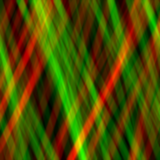
\includegraphics[width=2.5cm]{sources}}
  \centerline{(a)}
\end{minipage}
\begin{minipage}[b]{0.32\linewidth}
  \centering
  \centerline{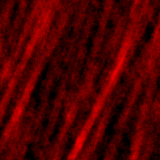
\includegraphics[width=2.5cm]{recon_focus1}}
  \centerline{(b)}
\end{minipage}
\begin{minipage}[b]{0.32\linewidth}
  \centering
  \centerline{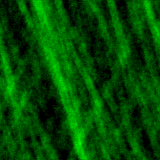
\includegraphics[width=2.5cm]{recon_focus2}}
  \centerline{(c)}
\end{minipage}

\begin{minipage}[b]{0.32\linewidth}
  \centering
  \centerline{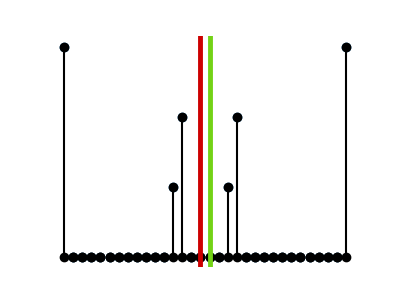
\includegraphics[width=3.6cm]{csbs_copies}}
  \centerline{(d)}
\end{minipage}
\begin{minipage}[b]{0.32\linewidth}
  \centering
  \centerline{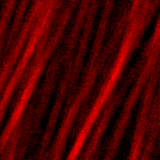
\includegraphics[width=2.5cm]{recon_csbs1}}
  \centerline{(e)}
\end{minipage}
\begin{minipage}[b]{0.32\linewidth}
  \centering
  \centerline{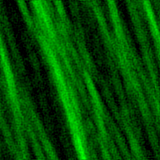
\includegraphics[width=2.5cm]{recon_csbs2}}
  \centerline{(f)}
\end{minipage}
\caption{(a) polychromatic source image with spectral components $\lambda_1$ and
  $\lambda_2$ (b) reconstruction of $\lambda_1$ from focal configuration (c)
  reconstruction of $\lambda_2$ from focal configuration (d) measurement
  locations selected by CSBS (e) reconstruction of
  $\lambda_1$ from CSBS configuration (f) reconstruction of $\lambda_2$ from
  CSBS configuration}
\label{fig:results}
\end{figure}

\begin{figure}[t]
\begin{minipage}[b]{0.23\linewidth}
  \centering
  \centerline{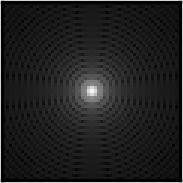
\includegraphics[width=2cm]{psf_focus1}}
  \centerline{(a)}
\end{minipage}
\begin{minipage}[b]{0.23\linewidth}
  \centering
  \centerline{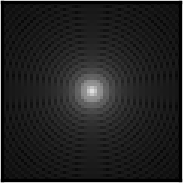
\includegraphics[width=2cm]{psf_focus2}}
  \centerline{(b)}
\end{minipage}
\begin{minipage}[b]{0.23\linewidth}
  \centering
  \centerline{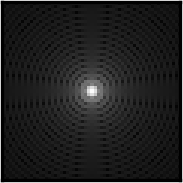
\includegraphics[width=2cm]{psf_csbs1}}
  \centerline{(c)}
\end{minipage}
\begin{minipage}[b]{0.23\linewidth}
  \centering
  \centerline{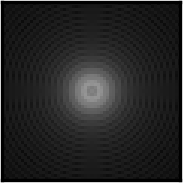
\includegraphics[width=2cm]{psf_csbs2}}
  \centerline{(d)}
\end{minipage}
\caption{(a) (b) PSFs at $\lambda_1$ focal plane. (c) (d) PSFs at a measurement location selected by CSBS
  (c) and (d) are less focused that (a) and (b), but have more measurement variation between them.
}
\label{fig:psfs_compare}
\end{figure}

% Figure \ref{fig:results}d shows the reconstructed image of the wavelength
% $\lambda_1$ with the 12 CSBS planes given in Figure \ref{fig:results}f and
% Figure \ref{fig:results}e shows the same with using 6 measurements in each focal
% plane. As can be seen from Figure \ref{fig:results} and Table \ref{tab:ssims},
% CSBS planes lead to better reconstruction than the focal planes. The reason why
% CSBS avoids focal planes is that the relative contribution from the off focus
% line are quite high at focal planes which degrades the reconstruction quality
% as the deconvolution cannot disentangle the spectral lines well.


% Finally, in Table \ref{tab:ssims}, we evaluate the error in the reconstructed
% spectral images using structural similary (SSIM) and peak signal-to-noise ratio
% (PSNR), where the CSBS reconstruction yielded better results measured by both metrics.
% \begin{table}[h]
% \caption{SSIM/PSNR comparison for CSBS vs focal planes}
% % \vspace{0.08 in}
% \centering
% \begin{tabular}{|c|c|c|}
% \hline
%       & Avg. SSIM  & Avg. PSNR  \\ \hline
% Focal & 0.347 & 9.53 dB \\ \hline
% CSBS  & 0.459 & 10.0 dB \\ \hline
% \end{tabular}
% \label{tab:ssims}
% \end{table}

\begin{figure}[htb]
  \begin{minipage}[b]{1\linewidth}
    \centering
    \centerline{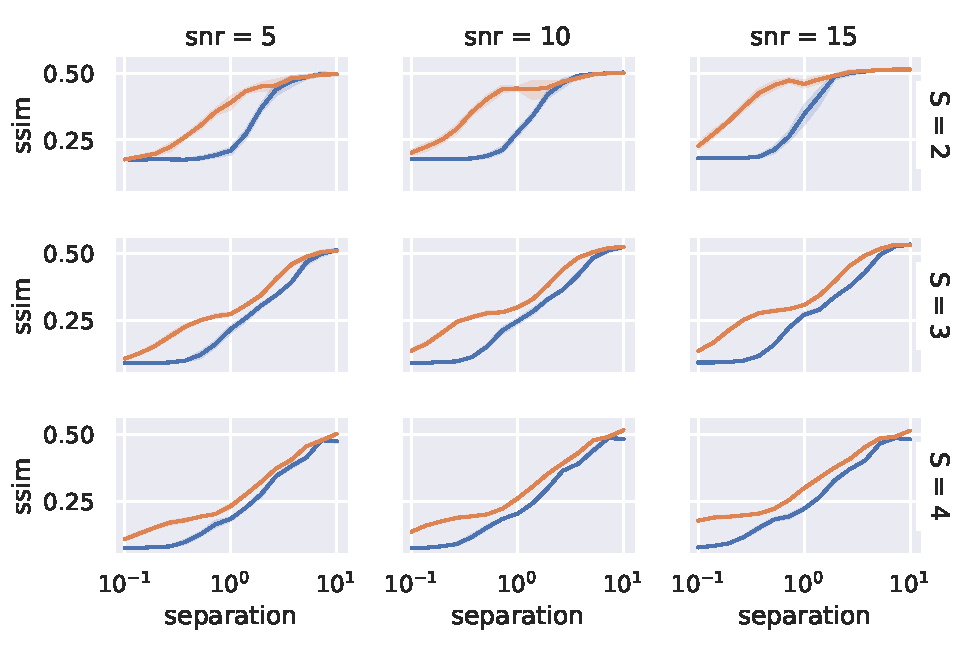
\includegraphics[width=8.5cm]{ssims}}
  \end{minipage}
  \caption{Reconstruction SSIMs for varied number of spectral components, SNR (dB), and source separation (DOF). CSBS reconstruction SSIM and
  focal plane reconstruction SSIM are shown in orange and blue, respectively.}
  \label{fig:ratio}
\end{figure}

To show that this reconstruction improvement generalizes, we repeat the first experiment for $S = 2, 3, 4$
uniformly spaced spectral components under different noise levels and
spectral component separations measured in depth of focus (DOF) \cite{davila2011high}.  In Figure \ref{fig:ratio}, we plot the mean
SSIM of the reconstructions obtained from measurements at focal planes (blue)
and measurements at planes selected by CSBS (orange).  The CSBS reconstructions
generally have higher SSIM than the focal plane up until the spectral components are sufficiently separated (about 10 DOF), where reconstruction SSIM are about the same.
\vspace{-0.1 in}
\section{Conclusion}
\vspace{-0.1 in}
We apply a variant of the sequential backward selection algorithm to the problem
of acquisition in a diffractive spectral imaging system.  The high
dimensionality of large images makes a direct application of CSBS and SSE cost
computationally intractable, so we have developed a more feasible implementation
of this algorithm and perform an analysis of its complexity to show that it is
significantly faster than the previous implementation for large images.
Finally, we demonstrate CSBS on a simulated spectral imaging system and show that
the optimized measurement configuration achieves equal or better reconstructions than a
choice of measurements at the spectral component focal planes.

\vfill\pagebreak
\clearpage

% References should be produced using the bibtex program from suitable
% BiBTeX files (here: strings, refs, manuals). The IEEEbib.bst bibliography
% style file from IEEE produces unsorted bibliography list.
% -------------------------------------------------------------------------
\bibliographystyle{IEEEbib}
\bibliography{bibliography}

\end{document}
